%
% NOTE -- ONLY EDIT THE .Rnw FILE!!!  The .tex file is
% likely to be overwritten.
%
% \VignetteIndexEntry{StepNorm Overview}
% \VignetteDepends{tools, MASS, marrayTools}
% \VignetteKeywords{Expression Analysis, Preprocessing}
% \VignettePackage{StepNorm}
\documentclass[11pt]{article}

\usepackage{amsmath,epsfig,fullpage}%,psfig,pstricks
\usepackage[authoryear,round]{natbib}
\usepackage{hyperref}
\usepackage{Sweave}

\parindent 0in

%\bibliographystyle{abbrvnat}

\newcommand{\code}[1]{{\tt #1}}
\newcommand{\Rfunc}[1]{{\tt #1}}
\begin{document}

\newcommand{\myincfig}[3]{%
  \begin{figure}[htbp]
    \begin{center}
      \includegraphics[width=#2]{#1}
      \caption{\label{#1}#3}
    \end{center}
  \end{figure}
}


\title{\bf Bioconductor's stepNorm package}

\author{Yuanyuan Xiao$^1$ and Yee Hwa Yang$^2$}

\maketitle


\begin{center}
Departments of $^1$Biopharmaceutical Sciences and $^2$Medicine \\
University of California, San Francisco\\ 
{\tt yxiao@itsa.ucsf.edu}\\
{\tt jean@biostat.ucsf.edu}
\end{center}

% library(tools)
%Rnwfile<- file.path("C:/Rpackages/StepNorm/StepNorm/inst/doc","stepNorm.Rnw")
% Sweave(Rnwfile,pdf=TRUE,eps=TRUE,stylepath=TRUE,driver=RweaveLatex())


\tableofcontents


%%%%%%%%%%%%%%%%%%%%%%%%%%%%%%%%%%%%%%%%%%%%%%%%%%%%%%%%%%%%%%%%%%%%%%%%%%%
\section{Overview}

This document provides a tutorial for the \code{stepNorm} package, which performs a 
stepwise within-slide normalization procedure STEPNORM on two-channel cDNA spotted arrays. 
Two-channel microarrays measure relative abundance of expression of thousands of genes 
in two mRNA populations. This relative abundance is usually expressed as ratios, 
$M = log_{2}\frac{R}{G}$, where $R$ and $G$ are the fluorescent intensity measurements 
of the red and green channels. The most pronounced systematic variation embodied in the 
ratios that does not contribute to differential expression between the two mRNA populations 
is the imbalance of the green and red dye incorporation. This imbalance is manifested as the 
dependence of ratios on primarily two factors, the fluorescent intensity ($A$) and the 
spatial heterogeneity ($S$).\\


STEPNORM is a normalization framework that integrates various models of different 
complexities to sequentially detect and adjust systematic variations associated with spot 
intensities ($A$), print-tips (PT), plates (PL) and two-dimensional spatial effects. 
For more details on STEPNORM, the reader is referred to \cite{stepNorm}. \\

{\bf Functionalities in \code{stepNorm}.} The \code{stepNorm} package implements the 
STEPNORM procedure which is based on a series of robust adaptive location normalization 
methods correcting for different types of dye biases (e.g. intensity, spatial, plate biases).
It enables the user to perform normalization either in a single-step or a sequential
fashion. Further, it allows the use of control sequences spotted onto the array and 
possibly spiked into the mRNA samples.\\

{\bf Microarray classes.} The \code{stepNorm} packages relies on microarray class definitions in 
{\tt marrayClasses}. You should also install this package and consult its vignette for more information.\\

{\bf Case study.} We demonstrate the functionality of the {\tt stepNorm} package using 
a \emph{swirl} zebrafish slide. The swirl experiment is comprised of four replicate 
hybridizations that contain 8,448 spots. It was carried out using zebrafish as a model 
organism to study the effect of a point mutation in the BMP2 gene that affects early 
development in vertebrates (\cite{NormNAR}). \\

{\bf Help files.}  As with any R package, detailed information on functions, classes and 
methods can be obtained in the help files. For instance, to view the help file for the 
function \Rfunc{stepWithinNorm} in a browser, use \code{help.start()} followed by 
\code{?stepWithinNorm}.\\


%%%%%%%%%%%%%%%%%%%%%%%%%%%%%%%%%%%%%%%%%%%%%%%%%%%%%%%%%%%%%%%%%%%%%%%%%%%
\section{Case study : The \emph{swirl} Experiment}

\subsection{Data}
We demonstrate the functionality of this package using gene expression
data from the \emph{swirl} experiment.  Two sets of dye-swap experiments 
were performed, for a total of four replicate hybridizations. For each 
of these hybridizations, target cDNA from the swirl mutant was labeled using one 
of the Cy3 or Cy5 dyes and the target cDNA wild-type mutant was labeled 
using the other dye. Target cDNA was hybridized to microarrays containing 
8,448 cDNA probes, including 768 controls spots (e.g. negative, positive, and
normalization controls spots). Microarrays were printed using 4
times 4 print-tips and are thus partitioned into a 4 times 4 grid
matrix. Each grid consists of a 22 times 24 spot matrix that was
printed with a single print-tip. Here, spot row and plate
coordinates should coincide, as each row of spots corresponds to
probe sequences from the same 384 well-plate. Raw images of the Cy3 and 
Cy5 fluorescence intensities for all four hybridizations are available at 
\url{http://fgl.lsa.berkeley.edu/Swirl/index.html}. To load the dataset, use
\code{data(swirl)}, and to view a description of the experiements
and data, type \code{?swirl}.


% begin code ----------------------------------------
\begin{Schunk}
\begin{Sinput}
> library(stepNorm)
\end{Sinput}
\begin{Soutput}
Loading required package: MASS 
Loading required package: marray 
\end{Soutput}
\begin{Sinput}
> data(swirl)
> maNsamples(swirl)
\end{Sinput}
\begin{Soutput}
[1] 4
\end{Soutput}
\begin{Sinput}
> maNspots(swirl)
\end{Sinput}
\begin{Soutput}
[1] 8448
\end{Soutput}
\end{Schunk}
% end code -----------------------------------------

\subsection{Single-step Normalization}   

The \code{stepNorm} package provides the function 
\Rfunc{withinNorm} to conduct normalization in a single-step 
fashion. For instance, The following commands applies the 
scatter plot smoother $loess$ within each print-tip-group
on a \emph{swirl} slide.

% begin code ----------------------------------------
\begin{Schunk}
\begin{Sinput}
> lpt.swirl <- withinNorm(swirl[, 1], norm = "loessPrintTip")
\end{Sinput}
\end{Schunk}
% end code -----------------------------------------

The function \Rfunc{withinNorm} is a simple wrapper function provided
for users interested in conducting a set of standard normalization
methods with default parameters (though supplying user desired parameters
is also feasible); its functionalites will be elaborated in the next
section.\\

\subsection{Stepwise Normalization with a Model Selection Component}  

As biases are slide- and experiment-dependent, 
different slides may show different intensity and spatial trends. Using one 
model (step) to correct all biases in a slide or using the same model for 
different slides exhibiting different biases might not be adequate. The
function \Rfunc{stepWithinNorm} implements the normalization procedure STEPNORM, 
which integrates a number of models under the same framework and assesses 
their effectiveness via a quantitative criterion. Such a process is applied 
to each individual slide in an experiment so that data (slide) specificity 
could be achieved. Unlike single-step normalization methods, STEPNORM could 
avoid data under-fitting or over-fitting as it implements both bias detection 
and removal in the same context. The following command using the function
\Rfunc{stepWithinNorm} applies a default stepwise procedure, which adjusts
$A$, $PT$, $PL$ and Spatial biases in an ordered succession, on a $swirl$
slide. Appropriately, the STEPNORM procedure chooses $loess$, median shift and median
shift for the correction of the $A$, $PT$ and $PL$ biases respectively and deems 
spatial heterogeneity on the slide not significant enough to warrant adjustments. 
Diagnostic plots before and after each step of bias adjustment are shown
in Figure \ref{stepNorm-swirlPlot}.

% begin code ----------------------------------------
\begin{Schunk}
\begin{Sinput}
> step.swirl1 <- stepWithinNorm(swirl[, 1])
\end{Sinput}
\begin{Soutput}
Normalizing slide  1 ...

BIC of null model:  -5328.85 

step  1 -- wholeChipA :
BIC of methods ( med rlm loess ) are:  -10138.86 -11389.80 -12019.94 
chosen :  loess 

step  2 -- printTipA :
BIC of methods ( med rlm loess ) are:  -12278.60 -12120.52 -11695.52 
chosen :  med 

step  3 -- plateA :
BIC of methods ( med rlm loess ) are:  -12821.92 -12750.23 -12250.72 
chosen :  med 

step  4 -- wholeChipSpatial :
BIC of methods ( rlm2D loess2D aov2D spatialMed ) are:  -12789.12 -12674.70 -12212.33 -12657.82 
this normalization step is not necessary

Slide 1 normalization steps:  wholeChipA-loess-> printTipA-med-> plateA-med 
\end{Soutput}
\begin{Sinput}
> norm.swirl <- step.swirl1[[1]]
> step.swirl1[[2]]
\end{Sinput}
\begin{Soutput}
[[1]]
                 From    To  Deviance   Enp Penalty Criterion
null                         -5328.85  0.00          -5328.85
wholeChipA            loess -12064.00 +4.87    9.04 -12019.94
printTipA               med -12467.33   +16    9.04 -12278.60
plateA                  med -13209.57   +22    9.04 -12821.92
wholeChipSpatial            -13209.57 +0.00         -12821.92
\end{Soutput}
\end{Schunk}
% end code -----------------------------------------


% end code ------------------------------------------------------------

\subsection{Sequential Normalization.}  

In addition to the \Rfunc{stepWithinNorm}
which includes a model selection component, the \code{stepNorm} package
also provides a multi-step normalization function \Rfunc{seqWithinNorm}, which
conducts normalization in a user specified sequence without the heavy computation 
burden of choosing among models. For instance, the following command employs
\code{``loess''} for correction of the $A$ bias, and the global median shift (
\code{``median''}) for the $PT$ and $PL$ biases and no normalization (
\code{``none''}) on the spatial bias.
 
% begin code ----------------------------------------
\begin{Schunk}
\begin{Sinput}
> step.swirl1 <- seqWithinNorm(swirl[, 1], A = "loess", PT = "median", 
+     PL = "median", Spatial2D = "none")
\end{Sinput}
\begin{Soutput}
Normalizing slide  1 ...

Deviance of null model: -5328.85 
enp 	 Deviance 	 BIC 
4.87 	 -12064 	 -12019.94 
16 	 -12467.33 	 -12278.6 
22 	 -13209.57 	 -12821.92 
0 	 -13209.57 	 -12821.92 
\end{Soutput}
\end{Schunk}
% end code -----------------------------------------

\section{The \Rfunc{withinNorm} function}

The function \Rfunc{withinNorm} provides a series of single-step
standard normalization. It wraps around functions \Rfunc{fitWithin} and 
\Rfunc{fit2DWithin} and returns an object of class {\tt marrayNorm}.
It has three arguments
\begin{description}
  \item
    {\code{marraySet}:} Object of class \code{marrayRaw} and \code{marrayNorm} 
    containing intensity data for the batch of arrays to be normalized. 
  \item
    {\code{subset}:} A logical or numeric vector indicating the subset of points 
    used to fit the normalization model.
  \item
    {\code{norm}:} Character string specifying the normalization method. 
    Thirteen normalization procedures are available with this function: \\
    \code{none},   no normalization; \\
    \code{median},   global median location normalization; \\ 
    \code{rlm},   global intensity or $A$--dependent robust linear 
    normalization; \\
    \code{loess},   global intensity or $A$--dependent robust nonlinear normalization; \\
    \code{medianPrintTip},   within-print-tip-group median normalization; \\
    \code{rlmPrintTip},   within-print-tip-group $rlm$ normalization; \\
    \code{loessPrintTip},   within-print-tip-group $loess$ normalization; \\
    \code{medianPlate},   within-well-plate-group median normalization; \\
    \code{rlmPlate},   within-well-plate-group $rlm$ normalization; \\
    \code{loessPlate},   within-well-plate-group $loess$ normalization; \\
    \code{aov2D},   spatial bivariate location normalization using ANOVA (\cite{Sellersetal03}); \\
    \code{rlm2D},   spatial bivariate location normalization using the \code{rlm} function; \\
    \code{loess2D},   spatial bivariate location normalization using the \code{loess} function; \\
    \code{spatialMedian},   spatial location normalization using a spatial median approach (\cite{Wilsonetal03}).
  \item
    {\code{$\dots$}:} Misc arguements for the specified 'norm' function
\end{description}
 
The function \Rfunc{withinNorm} is simple to use, the user needs only to input the
data as a \code{marrayRaw} (or \code{marrayNorm}) object and indicate the normalization 
method intended as a character string. It is also flexible to change parameters. For
example the default $loess$ normalization procedure uses $span = 0.4$, if a smaller span
is desired, it can be specified as follows, 

% begin code ----------------------------------------
\begin{Schunk}
\begin{Sinput}
> lpt.swirl <- withinNorm(swirl[, 1], norm = "loess", span = 0.2)
\end{Sinput}
\end{Schunk}
% end code -----------------------------------------   

The user should consult the functions \Rfunc{fitWithin} and \Rfunc{fit2DWithin} (using
\code{?fitWithin} and \code{?fit2DWithin}) for details on extra parameters suited for
each normalization method.
 

\section{The \Rfunc{stepWithinNorm} function}

The \Rfunc{stepWithinNorm} is the main function that carries out the 
STEPNORM procedure which adjusts biases sequentially and in a stepwise
normalization. In each step one bias is targeted for correction. Figure
\ref{fig:procedure} illustrates default steps by \Rfunc{stepWithinNorm},
which follows the successive correction of intensity (A), print-tip (PT), plate (PL) 
and spatial heterogeneity (2D Spatial) biases. Within each step several
models are employed competitively and the model that achieves the best
balance between the goodness of fit and simplicity is chosen for application
before proceeding to the next step. The \code{stepNorm} pacakge implement
two model selection criteria, the Akaike Information Criterion (AIC) and
the Bayesian Information Criterion (BIC). We recommend using the latter as
a typical microarray data consists of tens of thousands spots, and penalty
in BIC for number of model complexity is more appropriate for such big
datasets. \\

The function \Rfunc{stepWithinNorm} has four arguments (see also \code{?stepWitinNorm}): 
\begin{description}
  \item
    {\code{marrySet}:} Object of class \code{marrayRaw}or code{marrayNorm}, containing intensity 
    data for the batch of arrays to be normalized. 
  \item
    {\code{subset}:} A "logical" or "numeric" vector indicating the subset of points used to 
    compute the  normalization values.
  \item
    {\code{wf.loc}:} A list, each component of which is a step for the removal of a particular 
    systematic varation. Typically each step is also a list of several candidate models of 
    different complexity, such models can be specified using functions \Rfunc{fitWithin} and 
    \Rfunc{fit2DWithin} (see \code{?fitWithin} and \code{?fit2DWithin}). The function
    \Rfunc{makeStepList} is also provided for a user friendly approach to construct such a list;
    the user only needs to input the model names as character strings, see \code{?makeStepList}
    If missing, the default procedure will be used, which we consider appropriate for most slides
    (for details about the default procedure, see \code{?stepWithinNorm}).
  \item
    {\code{criterion}:} Character string specifying the criterion used for the selection of the
    best normalization procedure in each step. Choices include \code{``BIC''} and \code{``AIC''};
    if no specification is made, the default is \code{``BIC''}.
\end{description}

Normalization is performed simultaneously for each array in the batch using the same stepwise
procedure. We illustrate next on specifying customized stepwise procedure using the function
\Rfunc{makeStepList}. 
There may be cases when model selection for a certain step is not necessary, for example, when
the nonlinear trend between $M$ and $A$ is evident, the user may wish to apply $loess$ directly 
on the slide rather than enduring unnecessary computation on model comparisons. In addition, the
user desires no normalization on the Spatial 2D step. Such a procedure can be specified 
conveniently using the function \Rfunc{makeStepList}:

% begin code ----------------------------------------
\begin{Schunk}
\begin{Sinput}
> wf.loc <- makeStepList(A = "loess", Spatial2D = NULL)
> step.swirl1 <- stepWithinNorm(swirl[, 1], wf.loc = wf.loc)
\end{Sinput}
\begin{Soutput}
Normalizing slide  1 ...

BIC of null model:  -5328.85 

step  1 -- WholeChipA :
BIC of methods ( loess ) are:  -12019.94 
chosen :  loess 

step  2 -- PrintTipA :
BIC of methods ( median rlm loess ) are:  -12278.60 -12120.52 -11695.52 
chosen :  median 

step  3 -- PlateA :
BIC of methods ( median rlm loess ) are:  -12821.92 -12750.23 -12250.72 
chosen :  median 

Slide 1 normalization steps:  WholeChipA-loess-> PrintTipA-median-> PlateA-median 
\end{Soutput}
\end{Schunk}
% end code -----------------------------------------

However, \Rfunc{makeStepList} uses defalut parameters, for example, the span of 
$loess$ is set at 0.4 for the correction of the $A$ bias. To employ
parameters other than the defaults, the user needs to construct the \code{wf.loc}
list directly as the follows:

% begin code ----------------------------------------
\begin{Schunk}
\begin{Sinput}
> A <- list(loess = fitWithin(fun = "loessfit", span = 0.2))
> PT <- list(med = fitWithin(z.fun = "maPrintTip", fun = "medfit"), 
+     rlm = fitWithin(z.fun = "maPrintTip", fun = "rlmfit"), loess = fitWithin(z.fun = "maPrintTip", 
+         fun = "loessfit"))
> PL <- list(med = fitWithin(z.fun = "maCompPlate", fun = "medfit"), 
+     rlm = fitWithin(z.fun = "maCompPlate", fun = "rlmfit"), loess = fitWithin(z.fun = "maCompPlate", 
+         fun = "loessfit"))
> wf.loc <- list(wholeChipA = A, PrintTip = PT, Plate = PL)
> step.swirl1 <- stepWithinNorm(swirl[, 1], wf.loc = wf.loc)
\end{Sinput}
\end{Schunk}
% end code -----------------------------------------

 


\section{The \Rfunc{seqWithinNorm} function} 

The \Rfunc{seqWithinNorm} function allows the user to conduct a sequential 
normalization procedure without the heavy computational overhead of model
selection. The user can specify an appropriate model in each step or 
even skip a step. \\

The function \Rfunc{stepWithinNorm} has four arguments (see also \code{?stepWitinNorm}): 
\begin{description}
  \item
    {\code{marrySet}:} Object of class \code{marrayRaw} or \code{marrayNorm}, containing intensity 
    data for the batch of arrays to be normalized. 
  \item
    {\code{subset}:} A "logical" or "numeric" vector indicating the subset of points used to 
    fit the  normalization models.
  \item
    {\code{loss.fun}:} The loss function used in calucating deviance, the default uses squared 
    sum of residuals; for absolute sum of residuals, use \code{abs}.
  \item
    {\code{A}:}  A character string specifying the normalization method for the adjustment 
    of intensity or A bias; choices include \code{``median''}, \code{``rlm''}, \code{``loess''}
    and \code{``none''}. The default is set as \code{``loess''}.
  \item
    {\code{PT}:} A character string specifying the normalization method for the adjustment 
    of print-tip or PT bias; choices include \code{``median''}, \code{``rlm''}, \code{``loess''}
    and \code{``none''}. The default is set as \code{``median''}.
  \item
    {\code{PL}:} A character string specifying the normalization method for the adjustment 
    of well-plate or PL bias; choices include \code{``median''}, \code{``rlm''}, \code{``loess''}
    and \code{``none''}. The default is set as \code{``median''}.
  \item
    {\code{Spatial2D}:} A character string specifying the normalization method for the adjustment 
    of spatial 2D bias;  choices include \code{``rlm2D''}, \code{``aov2D''}, \code{``loess2D''},
    \code{``spatialMedian''} and \code{``none''}. The default is set as \code{``none'}. 
  \item
    {{criterion}:} Character string specifying the criterion, \code{``AIC''} or \code{``BIC''}.
    If no specification, \code{``BIC''} is used. Note that here criterion is calculated solely for 
    informaion purpose.
\end{description}

To conduct $loess$ normalization for the $A$ step, median normalization for the $PT$ step, and
no further normalization for the rest steps, the user can use the command below,

% begin code ----------------------------------------
\begin{Schunk}
\begin{Sinput}
> step.swirl1 <- seqWithinNorm(swirl[, 1], A = "loess", PT = "median", 
+     PL = "none", Spatial2D = "none")
\end{Sinput}
\begin{Soutput}
Normalizing slide  1 ...

Deviance of null model: -5328.85 
enp 	 Deviance 	 BIC 
4.87 	 -12064 	 -12019.94 
16 	 -12467.33 	 -12278.6 
0 	 -12467.33 	 -12278.6 
0 	 -12467.33 	 -12278.6 
\end{Soutput}
\end{Schunk}
% end code -----------------------------------------

%%%%%%%%%%%%%%%%%%%%%%%%%%%%%%%%%%%%%%%%%%%%%%%%%%%%%%%%%%%%%%%%%%%%%%%%%%%
\begin{thebibliography}{}

\bibitem[Sellers et~al.(2003)Sellers, Miecznikowski, and Eddy]{Sellersetal03}
K.~F. Sellers, J.~Miecznikowski, and W.~F. Eddy.
\newblock Removal of systematic variation in genetic microarray data.
\newblock Technical report, Department of Statistics, Carnegie Mellon
  University, 2003.

\bibitem[Wilson et~al.(2003)Wilson, Buckley, Helliwell, and
  Wilson]{Wilsonetal03}
D.~L. Wilson, M.~J. Buckley, C.~A. Helliwell, and I.~W. Wilson.
\newblock New normalization methods for cdna microarray data.
\newblock \emph{Bioinformatics}, 19:\penalty0 1325--1332, 2003.

\bibitem[Yang et~al.(2002)Yang, Dudoit, Luu, Lin, Peng, Ngai, and
  Speed]{NormNAR}
Y.~H. Yang, S.~Dudoit, P.~Luu, D.~M. Lin, V.~Peng, J.~Ngai, and T.~P. Speed.
\newblock Normalization for c{DNA} microarray data: a robust composite method
  addressing single and multiple slide systematic variation.
\newblock \emph{Nucleic Acids Research}, 30\penalty0 (4):\penalty0 e15, 2002.

\bibitem[Xiao et~al.(2004)Xiao, Segal, and Yang]{stepNorm}
Y.~Xiao, M.~R. Segal, and Y.~H. Yang.
\newblock Stepwise normalization of two-channel c{DNA} microarrays.
\newblock \emph{manuscript in preparation}.

\end{thebibliography}


\myincfig{stepNorm-swirlPlot}{\textwidth}{Diagnostic plots before and after $A$, $PT$ and
$PL$ biases correction for the first \emph{swirl} slide} 

\myincfig{stepProcedure}{\textwidth}{STEPNORM procedures for the swirl experiment. The swirl slides have 16 print-tips, 22 well plates, 88 rows and 96 columns.}

%\begin{figure}[htb]
%\begin{center}
%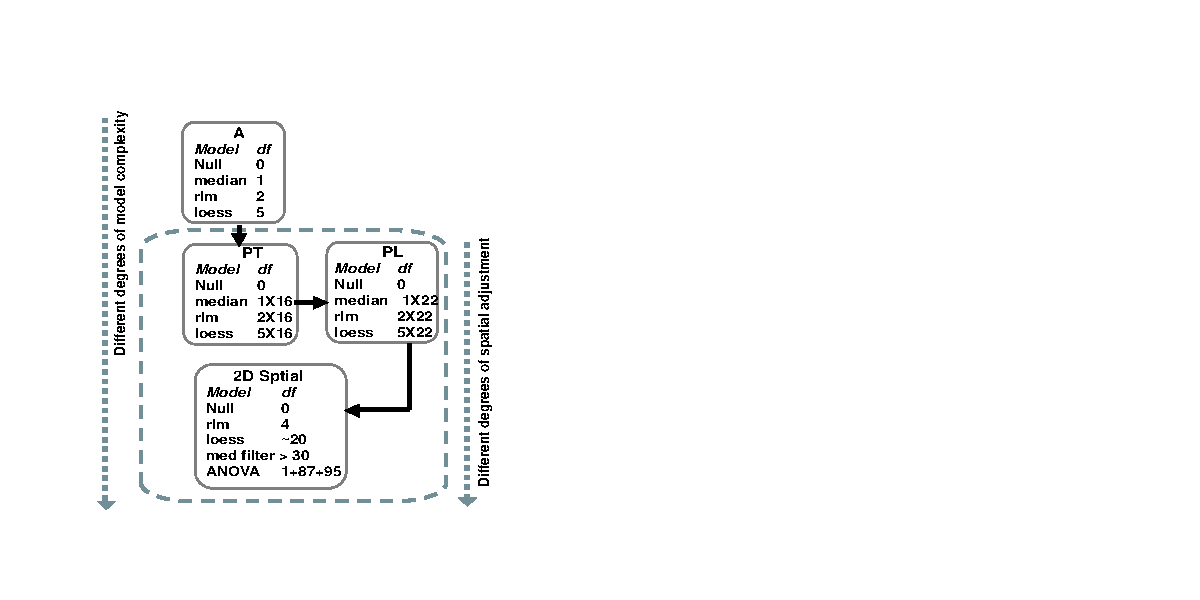
\epsfig{file=stepProcedure.eps, width=10cm}
%\end{center}
%\caption{STEPNORM procedures for the swirl experiment. The swirl slides have 16 print-tips, 22 well plates, 88 rows and 96 columns.}
%\label{fig:procedure}
%\end{figure}




%%%%%%%%%%%%%%%%%%%%%%%%%%%%%%%%%%%%%%%%%%%%%%%%%%%%%%%%%%%%%%%%%%%%%%%%%%%
\end{document}
 
